\documentclass{elsarticle}

\usepackage{amsmath}
\usepackage{hyperref}
\usepackage{subcaption}
\usepackage{tikz}     % for tikz pictures
\usetikzlibrary{calc} % for computing points in tikz pictures
\usetikzlibrary{shapes.geometric}

% equation punctuation
\newcommand{\eqp}{\,.} % equation period
\newcommand{\eqc}{\,,} % equation comma

% derivatives
\newcommand{\dd}[2]{\frac{d #1}{d #2}}               % ordinary derivative
\newcommand{\pd}[2]{\frac{\partial #1}{\partial #2}} % partial derivative
\newcommand{\ppt}[1]{\pd{#1}{t}}                     % partial d/dt
\newcommand{\ppx}[1]{\pd{#1}{x}}                     % partial d/dx
\newcommand{\ppy}[1]{\pd{#1}{y}}                     % partial d/dy
\newcommand{\ddt}[1]{\frac{d#1}{dt}}                 % ordinary d/dt

% phase-space arguments
\newcommand{\x}{\mathbf{x}}
\newcommand{\di}{\mathbf{\Omega}}
\newcommand{\xt}{(\x,t)}
\newcommand{\xet}{(\x,E,t)}
\newcommand{\xdet}{(\x,\di,E,t)}

% transport quantities
\newcommand{\aflux}{\psi}
\newcommand{\totalxsec}{\Sigma_\textup{t}}
\newcommand{\scatteringxsec}{\Sigma_\textup{s}}
\newcommand{\fissionxsec}{\Sigma_\textup{f}}
\newcommand{\Qext}{Q_\textup{ext}}
\newcommand{\Qtot}{Q_\textup{tot}}

% domain
\newcommand{\domain}{\mathcal{D}}
\newcommand{\normalvector}{\mathbf{n}}
\newcommand{\incoming}{u^{\textup{inc}}}

% linear system
\newcommand{\U}{\mathbf{U}}
\newcommand{\A}{\mathbf{A}}
\newcommand{\ssrhs}{\mathbf{b}}
\newcommand{\M}{\mathbf{M}}
\newcommand{\dt}{\Delta t}

% integrals and sums
\newcommand{\sumj}{\sum\limits_j}
\newcommand{\intSi}{\int\limits_{S_i}}
\newcommand{\intSij}{\int\limits_{S_{i,j}}}

% FEM
\newcommand{\test}{\varphi}

\newcommand{\tcr}[1]{\textcolor{red}{#1}}

\begin{document}
%------------------------------------------------------------------------------
\begin{frontmatter}

\journal{Journal of Computational and Applied Mathematics}

\title{Application of the Entropy Viscosity Method and the Flux-Corrected Transport
  Algorithm to the Particle Transport Equation using Continuous Finite Elements\\
	Flux-Corrected Transport Techniques Applied to the steady-state and time-dependent 
	Radiation Transport Equation discretized with CFEM	}

\author[tamu]{Joshua E. Hansel}
\ead{joshua.hansel89@gmail.com}

\author[tamu]{Jean C. Ragusa}
\ead{jean.ragusa@tamu.edu}

\address[tamu]{Texas A\&M University,
  400 Bizzell St,
  College Station, TX 77840}

\chapter*{ABSTRACT}
\addcontentsline{toc}{chapter}{ABSTRACT}

\pagestyle{plain} % No headers, just page numbers
%\pagenumbering{roman} % Roman numerals
\setcounter{page}{2}

\indent
The Flux-Corrected Transport (FCT) algorithm, in conjunction with the
entropy viscosity method, was applied with the continuous finite element method
to (a) a scalar transport equation that includes reaction and source terms and
(b) the shallow water equations.
For smooth problems, second-order spatial accuracy is achieved if adequate
solution bounds are used in the FCT algorithm. The resulting scheme is
positivity-preserving and reduces the onset of spurious oscillations.
Explicit SSPRK time discretizations are considered for both scalar
transport and the shallow water equations, and additionally
for scalar transport, $\theta$ time discretizations and
steady-state are considered. Explicit FCT schemes are shown to
be relatively robust; positivity preservation is guaranteed and spurious
oscillations are reduced, if not eliminated entirely.
Implicit/steady-state FCT schemes, however, are shown to have
significant nonlinear convergence issues in many cases, as is noted by
Kuzmin \cite{kuzmin_FCT}.

\pagebreak{}


\begin{keyword}
entropy viscosity \sep FCT \sep particle transport equation
\end{keyword}

\end{frontmatter}
%------------------------------------------------------------------------------
%\tcr{should we ask Guermond to be a 3rd author?}

\section{Introduction\label{sec:introduction}}
%================================================================================
\section{Introduction}
%================================================================================
The radiation transport equation is the following:
\begin{equation}\label{tr}
	\frac{1}{c}\frac{\partial \psi}{\partial t} + \mathbf{\Omega}\cdot\nabla\psi(\mathbf{x},t)
      + \sigma(\mathbf{x})\psi(\mathbf{x},t) = q(\mathbf{x},t),
\end{equation}
where $\psi(\mathbf{x},t)$ is the angular flux at position $\mathbf{x}$ and time
$t$ in direction $\mathbf{\Omega}$, $c$ is the transport speed, $\sigma(\mathbf{x})$
is the \emph{macroscopic} cross-section, and $q(\mathbf{x},t)$ is the
total source (extraneous plus scattering).
The problem definition is completed with an incoming flux boundary condition:
\begin{equation}
   \psi(\mathbf{x}) = \psi^{inc}(\mathbf{x})  \quad \forall \mathbf{x}\in \partial V^-,
      \quad \partial V^- = \{\mathbf{x}\in\partial V: \mathbf{\Omega}\cdot\mathbf{n}(\mathbf{x})<0\}.
\end{equation}
For transient problems, the following initial condition applies:
\begin{equation}
   \psi(\mathbf{x},t) = \psi^0(\mathbf{x})  \quad \forall \mathbf{x}\in V.
\end{equation}

\section{Preliminaries\label{sec:preliminaries}}
For the remainder of this paper, the scalar transport model given by
Equation~\eqref{eq:transport_scalar} will be generalized to a scalar
balance equation having reaction terms and source terms, with the following
notation:
\begin{equation}\label{eq:scalar_model}
  \ppt{u} + v\di\cdot\nabla u\xt
    + \sigma(\x) u\xt = q\xt
  \eqc
\end{equation}
where $u$ is the balanced quantity, $v$ is the transport speed, $\di$ is
a constant, uniform unit direction vector, $\sigma$ is the reaction coefficient,
and $q$ is the source function. Note that $q \ge 0$ for particle transport: the
external source, the inscattering source, and the fission source are all particle
production terms and hence are positive. 

The problem formulation is completed by supplying initial conditions on the
problem domain $\domain$ (for transient problems):
\begin{equation}
  u(\x,0) = u^0(\x) \quad \x\in\domain \eqc
\end{equation}
as well as boundary conditions,
which will be assumed to be incoming flux boundary conditions:
\begin{equation}
  u\xt = \incoming\xt \quad \x\in\partial\domain^- \eqc
\end{equation}
where $\incoming\xt$ is the incoming boundary data function, and
$\partial\domain^-$ is the incoming portion of the domain boundary:
\begin{equation}
  \partial\domain^- \equiv \{ \x\in\partial\domain :
  \normalvector(\x)\cdot\di \leq 0 \} \eqc
\end{equation}
where $\normalvector(\x)$ is the outward-pointing normal vector on the domain
boundary at point $\x$.

Application of the standard Galerkin method with piecewise linear basis functions
gives the following semi-discrete system:
\begin{subequations}\label{eq:galerkin_semidiscrete}
  \begin{equation}
    \M^C\ddt{\U} + \A\U(t) = \ssrhs(t) \eqc
  \end{equation}
where the consistent (i.e., not lumped) mass matrix is given by
  \begin{equation}
    M^C_{i,j} \equiv \intSij \test_i(\x)\test_j(\x) dV \eqc
  \end{equation}
the (steady-tstate) transport matrix is  
  \begin{equation}\label{eq:Aij}
    A_{i,j} \equiv \intSij\left(
    v\di\cdot\nabla\test_j(\x) +
    \sigma(\x)\test_j(\x)\right)\test_i(\x) dV \eqc
  \end{equation}
and the right-hand-side is
  \begin{equation}
    b_i(t) \equiv \intSi q(\x)\test_i(\x) dV \eqp
  \end{equation}
\end{subequations}
The components of the solution vector $\U(t)$ are denoted by $U_j(t)$ and represent
the degrees of freedom of the approximate solution $u_h$:
\begin{equation}
  u_h\xt = \sumj U_j(t) \test_j(\x) \eqc
\end{equation}
where $\test_j(\x)$ is a finite element test function.
$S_i$ is the support of basis function $i$ and $S_{i,j}$
is the shared support of basis functions $i$ and $j$.

A number of temporal discretizations are considered in this paper.
Fully explicit temporal discretizations considered include forward Euler:
\begin{equation}
  \M^C\frac{\U^{n+1}-\U^n}{\dt} + \A\U^n = \ssrhs^n \eqc
\end{equation}
as well as Strong Stability Preserving Runge Kutta (SSPRK) methods that
can be expressed in the following form:
\begin{subequations}\label{eq:ssprk}
\begin{align}
  & \hat{\U}^0 = \U^n \eqc \\
  & \hat{\U}^i = \gamma_i \U^n + \zeta_i \left[
      \hat{\U}^{i-1}
      + \dt\mathbf{G}(t^n+c_i\dt, \hat{\U}^{i-1})\right]
    \eqc \quad
    i = 1,\ldots,s
    \eqc \\
  & \U^{n+1} = \hat{\U}^s \eqp
\end{align}
\end{subequations}
where $s$ is the number of stages, $\gamma_i$, $\zeta_i$, and $c_i$ are
coefficients that correspond to the particular SSPRK method, and
$\mathbf{G}$ represents the right-hand-side function of an ODE
\begin{equation}
  \ddt{\U} = \mathbf{G}(t,\U(t)) \eqc
\end{equation}
which in this case is the following:
\begin{equation}
  \mathbf{G}(t,\U(t)) = (\M^C)^{-1}
    \left(\ssrhs(t) - \A\U(t)\right) \eqp
\end{equation}
SSPRK methods are a subclass of Runge Kutta methods that offer high-order
accuracy while preserving stability \cite{gottlieb}\cite{macdonald}.
The form given in Equation \eqref{eq:ssprk} makes it clear that these
SSPRK methods can be expressed as a linear combination of steps resembling
forward Euler steps, with the only difference being that the explicit
time dependence of the source is not necessarily on the old time $t^n$ but
instead is on a stage time $t^n + c_i\dt$.
An example is the 3-stage, 3rd-order accurate SSPRK
method has the following coefficients:
\begin{equation}
  \gamma = \left[\begin{array}{c}
    0\\\frac{3}{4}\\\frac{1}{3}\end{array}\right]
  \eqc \quad
  \zeta = \left[\begin{array}{c}
    1\\\frac{1}{4}\\\frac{2}{3}\end{array}\right]
  \eqc \quad
  c = \left[\begin{array}{c}0\\1\\\frac{1}{2}\end{array}\right] \eqp
\end{equation}

This work also considers the Theta-family of temporal discretizations:
\begin{equation}
  \M^C\frac{\U^{n+1}-\U^n}{\dt} + \A((1-\theta)\U^n + \theta\U^{n+1})
  = (1-\theta)\ssrhs^n + \theta\ssrhs^{n+1} \eqc
\end{equation}
where $0\leq\theta\leq 1$ is the implicitness parameter. For example,
$\theta$ values of $0$, $\frac{1}{2}$, and $1$ correspond to forward Euler,
Crank-Nicohlson, and backward Euler discretizations, respectively.

Finally, in the case of a steady-state solve, we have the following system of equations:
\begin{equation}
  \A\U = \ssrhs \eqp
\end{equation}


\section{FCT Methodology Applied to Particle Transport\label{sec:methodology}}
Testing with each FEM basis function $\varphi_i(\mathbf{x})$ gives a linear system:

\begin{equation}\label{eq:semidiscrete}
      \mathbf{M}^C\frac{d\mathbf{U}}{dt}+\mathbf{A} \mathbf{U}(t) = \mathbf{b},
\end{equation}

To discretize Eqn.~\ref{eq:semidiscrete} in time, fully explicit
temporal discretization schemes are used, such as explicit Euler:

\begin{equation}\label{eq:exgalerkin}
   \mathbf{M}^C\frac{\mathbf{U}^{n+1}-\mathbf{U}^n}{\Delta t}
     + \mathbf{A}\mathbf{U}^n = \mathbf{b}^n.
\end{equation}

In this section, a graph-theoretic approach introduced by Guermond~\cite{guermond_firstorder}
is taken to define a monotonicity-preserving, positivity-preserving low-order
scheme that satisfies a discrete maximum principle. Specifically, the low-order operator
is obtained by adding the the following dissipative term (written below for  the $i$-th equation):

\begin{equation}\label{eq:viscousform}
\sum_{K \subset S_i} \sum_{j\in \mathcal{I}(K)} U_j\nu_K^L b_K(\varphi_j,\varphi_i) .
\end{equation}

\noindent
The following local bilinear form has been employed to define this low-order scheme:

\begin{equation}\label{eq:bilinearform}
      b_K(\varphi_j, \varphi_i) \equiv \left\{\begin{array}{l l}
         -\frac{1}{n_K - 1}|K| & i\ne j, \quad i,j\in \mathcal{I}(K),\\
         |K|                   & i = j,  \quad i,j\in \mathcal{I}(K),\\
         0                     & i\notin\mathcal{I}(K) \quad | \quad j\notin\mathcal{I}(K),
      \end{array}\right.
\end{equation}

\noindent
where $K$ is the cell, $|K|$ is the volume of cell $K$, $\mathcal{I}(K)\equiv \{j\in\{1,\ldots,N\}: |S_j\cap K|\ne 0\}$
is the set of indices corresponding to degrees of freedom in
the support of cell $K$, and $n_K \equiv \mbox{card}(\mathcal{I}(K))$.
The local low-order viscosity is also defined:

\begin{equation}
   \nu_K^L \equiv \max\limits_{i\ne j\in \mathcal{I}(K)}\frac{\max(0,A_{i,j})}
      {-\sum\limits_{T\subset S_{i,j}} b_T(\varphi_j, \varphi_i)},
\end{equation}

\noindent
where $A_{i,j}$ is the $i,j$th entry of the Galerkin steady-state
matrix given by Eqn.~\ref{eq:Aij}.
Adding the viscous form of Eqn.~\ref{eq:viscousform} to the Galerkin scheme given in
Eqn.~\ref{eq:exgalerkin} gives the linear system for the low-order scheme

\begin{equation}\label{eq:loworderscheme}
   \mathbf{M}^L\frac{\mathbf{U}^{L,n+1}-\mathbf{U}^n}{\Delta t}
      +\mathbf{A}^L\mathbf{U}^n = \mathbf{b},
\end{equation}

\noindent
where $\mathbf{M}^L$ is the lumped mass matrix,
$\mathbf{U}^{L,n+1}$ is the low-order solution at time $t^{n+1}$, and
$\mathbf{A}^L = \mathbf{A} + \mathbf{D}^L$ is the low-order steady-state matrix,
which is the Galerkin steady-state matrix $\mathbf{A}$ plus a low-order
artificial diffusion matrix $\mathbf{D}^L$, defined as follows:

\begin{equation}\label{eq:loworderD}
   D^L_{i,j} = \sum\limits_{K\subset S_{i,j}}\nu_K^L b_K(\varphi_j,\varphi_i).
\end{equation}

\noindent
If the CFL condition $\Delta t \leq \frac{m_i}{A_{i,i}^L}$
is satisfied for all $i$, where the shorthand $m_i\equiv M^L_{i,i}$ applies, then the explicit
low-order scheme given in Eqn. \ref{eq:loworderscheme} satisfies the following
discrete maximum principle:

\begin{equation}\label{eq:dmp}
   U_{\min,i}^n\left(1-\frac{\Delta t}{m_i}
      \sum\limits_j A^L_{i,j}\right)
      + \frac{\Delta t}{m_i}b_i\leq
   U_i^{L,n+1}\leq
   U_{\max,i}^n\left(1-\frac{\Delta t}{m_i}
      \sum\limits_j A^L_{i,j}\right)
      + \frac{\Delta t}{m_i}b_i\quad\forall i,
\end{equation}

\noindent
where $U_{\min,i}^n = \min\limits_{j\in \mathcal{I}(S_i)}U_j^n$,
$U_{\max,i}^n = \max\limits_{j\in \mathcal{I}(S_i)}U_j^n$
and $\mathcal{I}(S_i)$ is the set of indices of degrees of freedom in the
support of degree of freedom $i$. The proof of this discrete maximum
principle is given in Appendix \ref{ap:dmp}.

%---------------------------------------------------------------------
\subsection{High-Order Scheme}\label{sec:highorder}

In this section, a high-order scheme based on the concept of entropy
viscosity introduced by Guermond~\cite{guermond_ev} is described, which by itself
is not guaranteed to be monotonicity-preserving or positivity-preserving;
however, when used as a component of the flux-corrected transport scheme given in
the following section, the resulting scheme is positivity-preserving
and satisfies a discrete maximum principle. Alternatively, one could use
the inviscid Galerkin scheme given in Eqn.~\ref{eq:exgalerkin} as
the high-order scheme component in the flux-corrected transport algorithm,
as has been done in the past for FEM-FCT~\cite{kuzmin_book}; however,
in practice it has been found that the FCT solution may still
contain small oscillations and effects that deteriorate the quality of the solution.

This scheme uses the high-order entropy viscosity scheme given by
Guermond~\cite{guermond_secondorder}.
One first decides upon a convex entropy functional $E(u)$ such as $E(u)=\frac{1}{2}u^2$.
The entropy viscosity is designed to add viscosity in regions of entropy
production, such as in shocks or steep gradients, and avoid adding
viscosity elsewhere. This is achieved by computing the entropy viscosity
with an entropy residual:

\begin{equation}
   \nu^{E,n}_K = \frac{c_E R_K^n(u_h^n,u_h^{n-1})
      + c_J\max\limits_{F\in\partial K}J_F(u_h^n)}
      {\|E(u_h^n)-\bar{E}(u_h^n)\|_{L^\infty(\mathcal{D})}},
\end{equation}

\noindent
where $R_K^n(u_h^n,u_h^{n-1})$ is the entropy residual, $J_F(u_h^n)$
is the jump in entropy flux across face $F$ of cell $K$, $\bar{E}(u_h^n)$ is the average
entropy over the domain, and $c_E$ and $c_J$ are tunable normalization
parameters, usually $\sim 1$.
The entropy residual evaluated with explicit Euler is the following:

\begin{equation}
    R_K^n(u_h^n,u_h^{n-1}) = \left\|\frac{E(u_h^n)-E(u_h^{n-1})}{\Delta t^n}
      + \left.\frac{dE}{du}\right|_{u_h^n}\left[\mathbf{\Omega}\cdot\nabla u_h^n
      + \sigma u_h^n
      - q \right]\right\|_{L^\infty(K)},
\end{equation}

\noindent
where the $L^\infty(K)$ norm is approximated as the maximum of the norm operand evaluated
at each quadrature point on $K$.
The entropy flux jumps are also computed on each face $F$ on the boundary of $K$:

\begin{equation}
   J_F(u_h^n) = \|\mathbf{\Omega}\cdot
      \mathbf{n}_F[\![\partial_n E(u_h^n)]\!]\|_{L^\infty(F)},
\end{equation}

\noindent
where $\mathbf{n}_F$ is the outward unit vector for face $F$,
$[\![\cdot]\!]$ denotes the jump in flux, and
the $L^\infty(F)$ norm is approximated as the maximum of the norm operand evaluated
at each quadrature point on $F$.

Finally, the high-order viscosity $\nu^{H,n}_K = \min(\nu^{L}_K,\nu^{E,n}_K)$ at
time $t^n$ is computed as the minimum
of the low-order viscosity $\nu^{L}_K$ defined in Section \ref{sec:loworder} and
the entropy viscosity $\nu^{E,n}_K$. The high-order counterpart of the low-order
artificial diffusion matrix defined in Eqn.~\ref{eq:loworderD} uses the high-order viscosity
$\nu_K^{H,n}$ instead of the low-order viscosity:

\begin{equation}
   D^{H,n}_{i,j} = \sum\limits_{K\subset S_{i,j}}\nu_K^{H,n} b_K(\varphi_j,\varphi_i).
\end{equation}

\noindent
Similarly to the low-order scheme, a high-order steady-state matrix
$\mathbf{A}^{H,n} = \mathbf{A} + \mathbf{D}^{H,n}$ is
defined to be the sum of the Galerkin steady-state matrix $\mathbf{A}$ and the
high-order artificial diffusion matrix $\mathbf{D}^{H,n}$,
and the high-order scheme is the following:

\begin{equation}\label{eq:highorderscheme}
   \mathbf{M}^C\frac{\mathbf{U}^{H,n+1}-\mathbf{U}^n}{\Delta t}
      +\mathbf{A}^{H,n}\mathbf{U}^n = \mathbf{b},
\end{equation}

\noindent
where $\mathbf{U}^{H,n+1}$ denotes the high-order solution at time $t^{n+1}$.

%---------------------------------------------------------------------
\subsection{Flux-Corrected Transport Scheme}\label{sec:fct}

This section blends the low-order and high-order schemes given
in Sections \ref{sec:loworder} and \ref{sec:highorder}, respectively, to produce a scheme
that is high-order, positivity-preserving, DMP-satisfying,
and in practice, free of spurious oscillations.

The crux of the flux-corrected transport algorithm is that an
antidiffusive flux $\mathbf{f}$ is defined that corrects the
low-order scheme to produce the high-order scheme solution:

\begin{equation}\label{eq:fct_full}
   \mathbf{M}^L\frac{\mathbf{U}^{H,n+1}-\mathbf{U}^n}{\Delta t}
      + \mathbf{A}^L\mathbf{U}^n
      = \mathbf{b} + \mathbf{f}.
\end{equation}

\noindent
Combining Eqns. \ref{eq:fct_full} and \ref{eq:highorderscheme}
yields the definition of $\mathbf{f}$:

\begin{equation}\label{gtf}
   \mathbf{f} \equiv -(\mathbf{M}^C-\mathbf{M}^L)
      \frac{\mathbf{U}^{H,n+1}-\mathbf{U}^n}{\Delta t}
      +(\mathbf{D}^L-\mathbf{D}^H)\mathbf{U}^n.
\end{equation}
It is easy to note that with the definition of $\mathbf{f}$ given in Eqn.~\ref{gtf},
Eqn.~\ref{eq:fct_full} yields the high-order solution. 

\noindent
However, the antidiffusive flux is added in a limited fashion
such that physically-motivated
solution bounds are not violated. In this paper, these bounds
are chosen to be the bounds of the low-order scheme discrete
maximum principle, given by Eqn.~\ref{eq:dmp}. With the
low-order and high-order schemes given in this paper, it
is possible to decompose the antidiffusive flux going into
node $i$, $f_i$, into a combination of internodal antidiffusive
fluxes $F_{i,j}$ such that $f_i = \sum\limits_j F_{i,j}$.
Since $\mathbf{M}^C-\mathbf{M}^L$ and $\mathbf{D}^L-\mathbf{D}^H$ are symmetric
and feature zero row and column sums, a valid decomposition for $\mathbf{f}$ is

\begin{equation}
   F_{i,j} = -M_{i,j}^C(\frac{U^{H,n+1}_j-U^n_j}{\Delta t} - \frac{U^{H,n+1}_i-U^n_i}{\Delta t})
   + (D_{i,j}^L-D_{i,j}^H)(U^n_j - U^n_i).
\end{equation}

\noindent
Finally, the FCT scheme is the following, where the operator
$\mathcal{L}$ denotes the limiter operation:

\begin{equation}\label{eq:FCTscheme}
   \mathbf{M}^L\frac{\mathbf{U}^{n+1}-\mathbf{U}^n}{\Delta t}
      + \mathbf{A}^L\mathbf{U}^n
      = \mathbf{b} + \mathcal{L}[\mathbf{F}],
\end{equation}

\noindent
where $(\mathcal{L}[\mathbf{F}])_i = \sum\limits_j \alpha_{i,j}F_{i,j}$
and $\mathbf{U}^{n+1}$ is the FCT solution at time $t^{n+1}$. The
limiting coefficients $\alpha_{i,j}$ are given by the multidimensional
limiter of Zalesak~\cite{zalesak}:

\begin{equation}\label{eq:P_defs}
   P_i^+ \equiv \sum\limits_j\max(0,F_{i,j}) \qquad
   P_i^- \equiv \sum\limits_j\min(0,F_{i,j}),
\end{equation}
\begin{equation}\label{eq:Q_defs}
      Q_i^\pm \equiv m_i\frac{W_i^\pm-U_i^n}{\Delta t}
      + \sum\limits_j A_{i,j}^L U_j^n - b_i,
\end{equation}
\begin{equation}\label{eq:R_defs}
   R_i^\pm \equiv\left\{
      \begin{array}{l l}
         1                                          & P_i^\pm = 0\\
         \min\left(1,\frac{Q_i^\pm}{P_i^\pm}\right) & P_i^\pm \ne 0
      \end{array}
      \right.,
\end{equation}
\begin{equation}\label{eq:L_defs}
   \alpha_{i,j} \equiv\left\{
      \begin{array}{l l}
         \min(R_i^+,R_j^-) & F_{i,j} \geq 0\\
         \min(R_i^-,R_j^+) & F_{i,j} < 0
      \end{array}
      \right.,
\end{equation}

\noindent
where $W_i^\pm$ are the upper and lower discrete maximum principle bounds
given in Eqn.~\ref{eq:dmp}. The proof that this definition of limiting
coefficients $\alpha_{i,j}$
satisfies the discrete maximum principle is given in Appendix \ref{ap:fct_dmp}.
Note that the symmetry of the limited coefficients $\alpha_{i,j}=\alpha_{j,i}$ and
antisymmetric correction fluxes $F_{i,j}=-F_{j,i}$ make the FCT scheme conservative, since
the FCT scheme is merely the low-order scheme plus some equal-and-opposite source
terms.

\subsection{Low-Order Scheme\label{sec:low}}
\begin{itemize}
  \item definitions - graph-theoretic bilinear form, viscosity, scheme
  \item M-matrix
  \item positivity preservation
  \item local DMP
\end{itemize}

\subsection{High-Order Scheme\label{sec:high}}
% !TEX root = ../paper.tex

\begin{itemize}
  \item definitions - entropy residual, entropy viscosity, scheme
\end{itemize}

This section describes the entropy viscosity method applied to the scalar
PDE given by Equation \eqref{eq:scalar_model}. Recall that the entropy
viscosity method is to be used as the high-order scheme in the FCT algorithm,
instead of the standard Galerkin method, as has been done previously
\cite{kuzmin_FCT}.
Usage of the entropy viscosity method in the FCT algorithm ensures convergence
to the entropy solution \cite{guermond_secondorder}.

The entropy viscosity method has been applied to a number of PDEs
such as general scalar conservation laws of the form
\begin{equation}\label{eq:scalar_conservation_law}
  \ppt{u} + \nabla\cdot\mathbf{f}(u) = 0
\end{equation}
and the inviscid Euler equations \cite{guermond_ev}. The scalar model studied
in this paper does not fit into the category of scalar conservation laws;
instead, it is more accurately described as a \emph{balance} law, due to
the addition of the reaction term $\sigma u$ and source term $q$. Application
of entropy viscosity to this equation is novel in this work.

Since the weak form of the problem does not have a unique solution, one
must supply additional conditions called \emph{admissibility} conditions or
\emph{entropy} conditions to filter out spurious weak solutions, leaving
only the physical weak solution, often called the entropy solution.
A number of entropy conditions are valid, but usually the most convenient
entropy condition for use in numerical methods takes the form of an
\emph{entropy inequality}, such as the following, which is valid for the
general scalar conservation law given by Equation \eqref{eq:scalar_conservation_law}:
\begin{equation}
  \ppt{\eta(u)} + \nabla\cdot\mathbf{\Psi}(u) \leq 0 \eqc
\end{equation}
which holds for any convex entropy function $\eta(u)$ and associated entropy
flux $\mathbf{\Psi}(u) \equiv \int \eta'(u)\mathbf{f}'(u)du$.
If one can show that this inequality holds for an arbitrary
convex entropy function, then one proves it holds for all convex entropy
functions  \cite{leveque2002}\cite{guermond_ev}.
For the scalar PDE considered in this paper, the entropy inequality becomes
the following:
\begin{equation}
  \ppt{\eta(u)} + \nabla\cdot\mathbf{\Psi}(u) + \eta'(u)\sigma u - \eta'(u)q
    \leq 0 \eqp
\end{equation}
One can verify this inequality by multiplying the governing PDE by $\eta'(u)$
and applying reverse chain rule.

The entropy viscosity method enforces the entropy inequality by measuring
local entropy production and dissipating accordingly. In practice, one
defines the entropy residual:
\begin{equation}
  \mathcal{R} \equiv \ppt{\eta(u)} + \nabla\cdot\mathbf{\Psi}(u)
    + \eta'(u)\sigma u - \eta'(u)q \eqc
\end{equation}
which can be viewed as the amount of violation of the entropy inequality.
The entropy viscosity for an element $K$ is then defined to be proportional
to this violation, for example:
\begin{equation}
  \nu^\eta_K = \frac{c_\mathcal{R}\|\mathcal{R}(u_h)\|_{L^\infty(K)}}
    {\hat{\eta}_K}
    \eqc
\end{equation}
where $\hat{\eta}_K$ is a normalization constant with the units of entropy,
$c_\mathcal{R}$ is a proportionality constant that can be modulated for
each problem, and $\|\mathcal{R}(u_h)\|_{L^\infty(K)}$ is the maximum of the
entropy residual on element $K$. In addition to the entropy residual, it can
also be beneficial to measure the jump in the gradient of the entropy flux
across interfaces.
Note that given the definition of the entropy flux, the gradient of the entropy
flux is $\nabla\mathbf{\Psi}(u)=\nabla\eta(u)\mathbf{f}'(u)$. Then let
$\mathcal{J}_F$ denote the jump of the normal component of the entropy flux
gradient across face $F$:
\begin{equation}
  \mathcal{J}_F \equiv |\mathbf{f}'(u)\cdot\mathbf{n}_F|
    [\![\nabla\eta(u)\cdot\mathbf{n}_F]\!] \eqc
\end{equation}
where the double square brackets denote a jump quantity. Then define the
maximum jump on a cell:
\begin{equation}
  \mathcal{J}_K \equiv \max\limits_{F\in\mathcal{F}(K)} |\mathcal{J}_F| \eqp
\end{equation}
Finally, putting everything together, one can define the entropy viscosity
for a cell $K$ to be
\begin{equation}
  \nu^\eta_K = \frac{c_\mathcal{R}\|\mathcal{R}(u_h)\|_{L^\infty(K)}
    + c_\mathcal{J}\mathcal{J}_K}{\hat{\eta}_K}
    \eqp
\end{equation}
However, it is known that the low-order viscosity for an element, as computed
in Section \ref{sec:low}, gives enough local artificial diffusion for
regularization; any excess of this viscosity would be excessive and further
degrade spatial accuracy. Thus, the low-order viscosity for an element is
imposed as the upper bound for the high-order viscosity:
\begin{equation}
  \nu^H_K \equiv \min(\nu^L_K, \nu^\eta_K) \eqp
\end{equation}
One should see that in smooth regions, this high-order viscosity should be
relatively small, and in regions of strong gradients or discontinuities,
the entropy viscosity should be relatively large, ideally approximately
as large as the low-order viscosity. Note that the latter condition can
be achieved in part by tuning the tuning parameters
$c_\mathcal{R}$ and $c_\mathcal{J}$ for the particular problem.

\subsection{FCT Scheme\label{sec:fct}}
% !TEX root = ../paper.tex

\begin{itemize}
  \item solution bounds - characteristic (upwind and non-upwind)
  \item antidiffusion bounds - definition and requirements for fail-safe
  \item limiters - Zalesak, multi-pass?
\end{itemize}

\subsubsection{The FCT System}

The entropy viscosity method described in Section \ref{sec:high} enforces
the entropy condition and thus produces numerical approximations that
converge to the entropy solution. However, numerical solutions may still
contain spurious oscillations and negativities, although these effects are
smaller in magnitude than for the corresponding Galerkin solution.
In this paper, the flux-corrected transport (FCT) algorithm
is used to further mitigate the formation of spurious oscillations and
to guarantee the absence of negativities.

The first ingredient of the FCT algorithm is the definition of the antidiffusive
fluxes. To arrive at this definition, the low-order systems, given by Equations
\ref{eq:low_ss}, \ref{eq:low_fe}, and \ref{eq:low_theta} for each temporal
discretization, are augmented with the addition of the \emph{antidiffusion source}
$\p$, which now, instead of producing the low-order solution, produces the high-order
solution $U^H$.
\begin{equation}\label{eq:antidiffusionsource_ss}
  \A^L \U^H = \ssrhs + \p \eqc
\end{equation}
\begin{equation}\label{eq:antidiffusionsource_fe}
  \M^L\frac{\U^H - \U^n}{\dt} + \A^L\U^n = \ssrhs^n + \p \eqc
\end{equation}
\begin{equation}\label{eq:antidiffusionsource_theta}
  \M^L\frac{\U^H - \U^n}{\dt} + \A^L\pr{\theta\U^{n+1} + (1-\theta)\U^n}
    = \ssrhs^\theta + \p \eqp
\end{equation}
Then the corresponding high-order systems, given by Equations \ref{eq:high_ss},
\ref{eq:high_fe}, \ref{eq:high_theta} are subtracted from these equations
to give the following definitions for $\p$:
\begin{equation}\label{eq:antidiffusionsourcei_ss}
  \p \equiv \pr{\D^L - \D^H}\U^H \eqc
\end{equation}
\begin{equation}\label{eq:antidiffusionsourcei_fe}
  \p \equiv -\pr{\M^C - \M^L}\frac{\U^H - \U^n}{\dt} + \pr{\D^L - \D^H}\U^n \eqc
\end{equation}
\begin{multline}\label{eq:antidiffusionsourcei_theta}
  \p \equiv -\pr{\M^C - \M^L}\frac{\U^H - \U^n}{\dt}
    + (1-\theta)\pr{\D^L - \D^{H,n}}\U^n\\
    + \theta    \pr{\D^L - \D^{H,n+1}}\U^{n+1} \eqc
\end{multline}
The next step is to decompose each antidiffusive source $p_i$ into a sum of
antidiffusive fluxes: $p_i = \sum_j P_{i,j}$. Because the matrices $\M^C-\M^L$
and $\D^L-\D^H$ are symmetric and feature row sums of zero, the following
are valid antidiffusive flux decompositions:
\begin{equation}
  P_{i,j} = \pr{D^L_{i,j} - D^H_{i,j}}\pr{U^H_j - U^H_i} \eqc
\end{equation}
\begin{equation}
  P_{i,j} = -M^C_{i,j}\pr{\frac{U^H_j - U^n_j}{\dt} - \frac{U^H_i - U^n_i}{\dt}}
    + \pr{D^L_{i,j} - D^{H,n}_{i,j}}\pr{U^n_j - U^n_i}  \eqc
\end{equation}
\begin{multline}
  P_{i,j} = -M^C_{i,j}\pr{\frac{U^H_j - U^n_j}{\dt} - \frac{U^H_i - U^n_i}{\dt}}
    + (1-\theta)\pr{D^L_{i,j} - D^{H,n}_{i,j}}\pr{U^n_j - U^n_i}\\
    + \theta\pr{D^L_{i,j} - D^{H,n+1}_{i,j}}\pr{U^H_j - U^H_i} \eqp
\end{multline}
Note that this decomposition yields equal and opposite antidiffusive flux pairs
since the antidiffusion matrix $\P$ is skew symmetric: $P_{j,i}=-P_{i,j}$.
Up until this point, no changes have been made to the
high-order scheme, although it has been expressed in a different form.
To apply the FCT algorithm, limiting coefficients $L_{i,j}$ are applied to
each antidiffusive flux $P_{i,j}$. Thus the FCT systems are the following:
\begin{equation}\label{eq:fct_ss}
  \A^L \U^H = \ssrhs + \bar{p} \eqc
\end{equation}
\begin{equation}\label{eq:fct_fe}
  \M^L\frac{\U^H - \U^n}{\dt} + \A^L\U^n = \ssrhs^n + \bar{p} \eqc
\end{equation}
\begin{equation}\label{eq:fct_theta}
  \M^L\frac{\U^H - \U^n}{\dt} + \A^L\pr{\theta\U^{n+1} + (1-\theta)\U^n}
    = \ssrhs^\theta + \bar{p} \eqc
\end{equation}
where the overbar denotes limitation: $\bar{p}_i\equiv\sum_j L_{i,j}P_{i,j}$.
The limiting coefficients each range between zero and one, representing
full limitation and no limitation, respectively. Setting all limiting
coefficients to zero would result in the low-order solution, and setting
all to one would result in the high-order solution. The actual values of the
limiting coefficients are determined by the limiter, which operates on the
following goal: maximize the limiting coefficients such that the imposed
solution bounds are not violated.

%===============================================================================
% !TEX root = ../paper.tex

\subsubsection{Solution Bounds}\label{sec:solution_bounds}

\tcr{maybe a bit more transport meat to show how one obtains the integral form of the TE would be good here}

Solution bounds for the transport model given by Equation \eqref{eq:scalar_model}
can be derived using the integral transport equation \cite{Add_a_Ref}, which is obtained using
the method of characteristics:
\begin{multline}\label{eq:integral_transport}
   u(\x,t) = u_0(\x - v t\di) e^{-\int\limits_0^t
    \sigma(\x - v(t -t')\di)v dt'}\\
    + \int\limits_0^t q(\x - v(t -t')\di,t') e^{-\int\limits_{t'}^t
    \sigma(\x - v(t -{t''})\di)v d{t''}} v dt' \eqp
\end{multline}

% %================================================================================
% \section{Introduction}
% %================================================================================
% In this section, an analytic local maximum principle is derived for
% scalar conservation laws having a constant, linear flux $\consfluxscalar$,
% i.e., $\consfluxscalar = \velocity u$ with $\nabla\cdot(\velocity u) =
% \velocity\cdot\nabla u$, where $\velocity$ is the constant velocity field. This
% analysis is valid for radiation transport, where the constant velocity field is
% $\velocity=v\directionvector$, with $v$ being the radiation speed.
%
% The analytic DMPs are derived using the method of characteristics, whereby
% paths in the $x-t$ plane are found, along which the governing PDE becomes an ODE.
% This is simple for the case of constant linear transport because in this case
% the characteristics are constant.
%
% %================================================================================
% \section{Integral Form of the Linear Transport Equation}
% %================================================================================
% \begin{theorem}{Integral Form of the Linear Transport Equation}{}
%    An implicit solution to the initial value problem
%    \begin{equation}\label{PDE}
%      \frac{1}{v}\ppt{\scalarsolution}
%        + \directionvector\cdot\nabla\scalarsolution(\x,t)
%         + \sigma(\x)\scalarsolution(\x,t)
%         = q(\x,t),
%      \qquad \scalarsolution(\x,0) = \scalarsolution_0(\x)
%    \end{equation}
%    is the following:
%    \begin{equation}\label{eq:integral_form}
%       \scalarsolution(\x,t) = \scalarsolution_0(\x - v t\directionvector)
%          e^{-\int\limits_0^t \sigma(\x - v(t -t')\directionvector)v dt'} +
%          \int\limits_0^t q(\x - v(t -t')\directionvector,t')
%            e^{-\int\limits_{t'}^t\sigma(\x
%              - v(t -\bar{t})\directionvector)v d\bar{t}} v dt' \eqp
%    \end{equation}
% \end{theorem}
%
% \begin{proof}
%    This proof will proceed by using the method of characteristics. The position
%    $\x$ will be regarded as a function of time: $\x=\x(t)$.
%    The characteristic $\x(t)$ is the solution of the following initial value problem:
%    \[
%       \frac{d\x}{dt} = v\directionvector \eqc \qquad \x(0) = \x_0 \eqc
%    \]
%    which is
%    \[
%       \x(t) = \x_0 + v t\directionvector \eqp
%    \]
%    Taking the derivative of $\scalarsolution(\x(t),t)$ gives
%    \begin{eqnarray*}
%       \frac{d\scalarsolution}{dt} & = &\ppt{\scalarsolution}
%         + \nabla\cdot\scalarsolution(\x(t),t) \frac{d\x}{dt}\\
%         & = & \ppt{\scalarsolution}
%         + v\directionvector\cdot\nabla\scalarsolution(\x(t),t) \eqc
%    \end{eqnarray*}
%    which when combined with the PDE in Equation \eqref{PDE}, gives
%    \begin{equation}\label{eq:pre_integrating_factor}
%       \ddt{\scalarsolution} + v\sigma(\x(t))\scalarsolution(\x(t),t)
%         = vq(\x(t),t) \eqp
%    \end{equation}
%    This is a 1st-order linear ODE, which may be solved using an integrating factor
%    \[
%       \mu(t)=e^{\int\limits_0^t\sigma(\x(t'))v dt'}.
%    \]
%    Multiplying both sides of Equation \eqref{eq:pre_integrating_factor}
%    by this integrating factor and using the product rule,
%    \[
%       \frac{d}{dt}\left[\scalarsolution(\x(t),t)\mu(t)\right]
%         = vq(\x(t),t) \mu(t) \eqc
%    \]
%    and integrating from $0$ to $t$ gives
%    \[
%       \scalarsolution(\x(t),t)\mu(t)-\scalarsolution(\x(0),0)\mu(0) =
%          \int\limits_0^t q(\x(t'),t') \mu(t') v dt' \eqp
%    \]
%    Simplifying,
%    \[\begin{split}
%       \scalarsolution(\x(t),t) &= \scalarsolution(\x(0),0)
%          e^{-\int\limits_0^t \sigma(\x(t'))v dt'} +
%          \left(\int\limits_0^t q(\x(t'),t')
%            e^{\int\limits_0^{t'}\sigma(\x(\bar{t}))v d\bar{t}}
%            v dt'\right)
%          e^{-\int\limits_0^tv\sigma(\x(t'))dt'} \eqc\\
%       &= \scalarsolution(\x(0),0)
%          e^{-\int\limits_0^t \sigma(\x(t'))v dt'} +
%          \int\limits_0^t q(\x(t'),t')
%            e^{-\int\limits_{t'}^t\sigma(\x(\bar{t}))v d\bar{t}}
%            v dt' \eqp
%    \end{split}\]
%    Finally, expressing $\x(t)$ in terms of $\x$, $v$, $\directionvector$,
%    and $t$ gives
%    \begin{multline*}
%       \scalarsolution(\x,t) = \scalarsolution_0(\x - v t\directionvector)
%          e^{-\int\limits_0^t \sigma(\x - v(t -t')\directionvector)
%            v dt'}\\
%          + \int\limits_0^t q(\x - v(t -t')\directionvector,t')
%            e^{-\int\limits_{t'}^t\sigma(\x
%              - v(t -\bar{t})\directionvector)v d\bar{t}}
%              v dt'\eqp \qed
%    \end{multline*}
% \end{proof}
% %================================================================================
% \section{Local Maximum Principles\label{sec:local_max_principles}}
% %================================================================================
% Before giving an analytic local discrete maximum principle, a local maximum
% principle applying to a general region is given by the following theorem.
%
% \begin{theorem}[thm:analytic_max_principle]{Analytic Local Maximum Principle}
%    Let $L(\x,\tau)$ be the line segment that spans between
%    $\x-v\tau\directionvector$ and $\x$:
%    \begin{equation}
%       L(\x,\tau)\equiv \left\{\mathbf{y}\in\mathbb{R}^d : \mathbf{y}
%          = \x-v t\directionvector \eqc \qquad t\in(0,\tau) \right\} \eqp
%    \end{equation}
%    See Figure \ref{fig:neighborhood} for an illustration.
%    The following local maximum principle is valid for the solution to the
%    problem given by Equation \eqref{PDE}:
%    \begin{subequations}\label{eq:local_max_principle}
%    \begin{equation}
%       \scalarsolution_{\text{min}} \le \scalarsolution(\x,\tau)
%         \le \scalarsolution_{\text{max}} \eqc
%    \end{equation}
%    \begin{equation}
%       \scalarsolution_{\text{min}}
%         \equiv \left\{\begin{array}{l l}
%           %\scalarsolution_{\min,N}^0
%           \scalarsolution_0(\x - v \tau\directionvector)
%              e^{-v\tau\sigma_{\max,L}}
%             + \frac{q_{\min,L}}{\sigma_{\max,L}}
%              (1 - e^{-v\tau\sigma_{\max,L}}) \eqc
%           & \sigma_{\max,L} \ne 0 \\
%           %\scalarsolution_{\min,L}^0
%           \scalarsolution_0(\x - v \tau\directionvector)
%             + v\tauq_{\min,L} \eqc
%           & \sigma_{\max,L} = 0
%         \end{array}\right.\eqc
%    \end{equation}
%    \begin{equation}
%       \scalarsolution_{\text{max}}
%         \equiv \left\{\begin{array}{l l}
%           %\scalarsolution_{\max,N}^0
%           \scalarsolution_0(\x - v \tau\directionvector)
%             e^{-v\tau\sigma_{\min,L}}
%             + \frac{q_{\max,L}}{\sigma_{\min,L}}
%             (1 - e^{-v\tau\sigma_{\min,L}}) \eqc
%           & \sigma_{\min,L} \ne 0 \\
%           %\scalarsolution_{\max,N}^0
%           \scalarsolution_0(\x - v \tau\directionvector)
%             + v\tauq_{\max,L} \eqc
%           & \sigma_{\min,L} = 0
%         \end{array}\right.\eqc
%    \end{equation}
%    \begin{equation}
%      \sigma_{\min,L}\equiv\min\limits_{\mathbf{y}\in L(\x,\tau)}
%        \sigma(\mathbf{y}) \eqc \quad
%      \sigma_{\max,L}\equiv\max\limits_{\mathbf{y}\in L(\x,\tau)}
%        \sigma(\mathbf{y}) \eqc
%    \end{equation}
%    \begin{equation}
%      q_{\min,L}\equiv\min\limits_{\mathbf{y}\in L(\x,\tau)}
%        q(\mathbf{y}) \eqc \quad
%      q_{\max,L}\equiv\max\limits_{\mathbf{y}\in L(\x,\tau)}
%        q(\mathbf{y}) \eqp
%    \end{equation}
%    \end{subequations}
% \end{theorem}
% %-------------------------------------------------------------------------------
% \begin{figure}[htb]
%    \centering
%      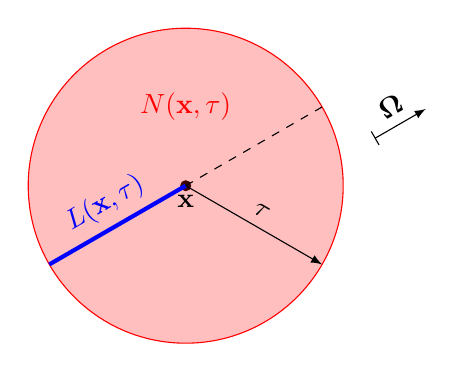
\begin{tikzpicture}[
  scale=1]

\def\pointsize{2pt}
\def\radius{2}

\coordinate (mycenter) at (0,0);
\fill (mycenter) circle (\pointsize);
\draw[draw=red, fill=red, fill opacity=0.25] (mycenter) circle (\radius);
\draw (mycenter) node[below] {$\x$};
\draw[-latex] (mycenter) -- (-30:\radius) node[pos=0.5,sloped,above] {$\speed\tau$};
\draw[blue,line width=1.5pt] (mycenter) -- (210:\radius)
  node[pos=0.5,sloped,above] {$L(\x,\tau)$};
\draw[dashed] (mycenter) -- (30:\radius);
\node[red] at ($0.5*(0,\radius)$) {$N(\x,\tau)$};
\coordinate (dircenter) at (1.2*\radius,0.3*\radius);
\draw[|-latex,shift=(dircenter)] (0,0) -- (30:0.75)
  node[pos=0.5,sloped,above] {$\di$};

\end{tikzpicture}

%       \caption{Illustration of Neighborhoods $L(\x,\tau)$ and $N(\x,\tau)$}
%    \label{fig:neighborhood}
% \end{figure}
% %-------------------------------------------------------------------------------
% \begin{proof}
%    Rewriting Equation \eqref{eq:integral_form} with $t=\tau$ gives
%    \begin{multline*}
%       \scalarsolution(\x,\tau) = \scalarsolution_0(\x - v\tau\directionvector)
%          e^{-\int\limits_0^\tau \sigma(\x
%            - v(\tau -t')\directionvector)v dt'}\\
%          +
%          \int\limits_0^\tau q(\x - v(\tau -t')\directionvector,t')
%          e^{-\int\limits_{t'}^\tau \sigma(\x
%          - v(\tau -\bar{t})\directionvector)v d\bar{t}}v dt' \eqp
%    \end{multline*}
%    One can bound the first term in the right-hand-side of Equation
%    \eqref{eq:integral_form} by considering
%    the maximum and minimum cross section on the line segment $L(\x,\tau)$
%    for the lower and upper bounds, respectively:
%    \[
%       %\scalarsolution_{\min,L}^0
%       \scalarsolution_0(\x - v\tau\directionvector)
%         e^{-v\tau\sigma_{\max,L}} \le
%       \scalarsolution_0(\x - v\tau\directionvector)
%         e^{-\int\limits_0^\tau \sigma(\x
%            - v(\tau -t')\directionvector)v dt'} \le
%       %\scalarsolution_{\max,L}^0
%       \scalarsolution_0(\x - v\tau\directionvector)
%         e^{-v\tau\sigma_{\min,L}} \eqp
%    \]
%    The source term can be bounded as follows:
%    \begin{align*}
%      \scalarsolution_q
%       & \equiv
%          \int\limits_0^\tau q(\x - v(\tau -t')\directionvector,t')
%          e^{-\int\limits_{t'}^\tau \sigma(\x
%            - v(\tau -\bar{t})\directionvector)v d\bar{t}} v dt'\\
%       & \le
%          q_{\max,L}\int\limits_0^\tau
%          e^{-\int\limits_{t'}^\tau \sigma(\x
%            - v(\tau -\bar{t})\directionvector)v d\bar{t}}v dt'\\
%       & \le
%          q_{\max,L}\int\limits_0^\tau
%          e^{-\sigma_{\min,L}\int\limits_{t'}^\tau v d\bar{t}}v dt'\\
%       & =
%          q_{\max,L} \int\limits_0^\tau
%          e^{-v(\tau-t')\sigma_{\min,L}}v dt'\\
%       & =
%          q_{\max,L}e^{-v\tau\sigma_{\min,L}}
%          \int\limits_0^\tau e^{\sigma_{\min,L}v t'}v dt'\\
%       & =
%          \left\{\begin{array}{l l}
%             \frac{q_{\max,L}}{\sigma_{\min,L}}
%               (1 - e^{-v\tau\sigma_{\min,L}}) \eqc
%                & \sigma_{\min,L} \ne 0\\
%             v\tau q_{\max,L} \eqc & \sigma_{\min,L} = 0
%             \end{array}\right.
%    \end{align*}
%    A similar analysis is performed for the lower bound.
%    Putting the two components together gives the bounds given by Equation
%    \eqref{eq:local_max_principle}.\qed
% \end{proof}
% %-------------------------------------------------------------------------------
%
% This result gives relatively tight solution bounds; however, its use as
% solution bounds for FCT may prove difficult in practice (especially for
% multi-dimensional problems), as one must
% compute the solution at the point $\x-v\tau\di$ and must be able
% to evaluate the minimum and maximum of the reaction coefficients and
% sources on the line segment $L(\x_i,\tau)$.
% The following corollary loosens the solution bounds for use in a
% more simple implementation of solution bounds for FCT. It considers
% not just the upstream line segment of length $v\tau$, but the
% sphere of radius $v\tau$ centered at $\x_i$.
%
% %-------------------------------------------------------------------------------
% \begin{corollary}[cly:loose_analytic_max_principle]
%   {Loose Analytic Local Maximum Principle}
% Let $N(\x,\tau)$ denote the sphere centered at $\x$ with radius
% $v\tau$, as shown in Figure \ref{fig:neighborhood}:
%    \begin{equation}\label{eq:neighborhood}
%       N(\x,\tau)\equiv\left\{\mathbf{y}\in\mathbb{R}^d :
%          \|\mathbf{y} - \x\| \le v\tau\right\} \eqp
%    \end{equation}
% The following, looser, local maximum principle is valid for the solution to the
% problem given by Equation \eqref{PDE}:
% \begin{subequations}\label{eq:loose_local_max_principle}
%    \begin{equation}
%       \scalarsolution_{\text{min}} \le \scalarsolution(\x,\tau)
%         \le \scalarsolution_{\text{max}} \eqc
%    \end{equation}
%    \begin{equation}
%       \scalarsolution_{\text{min}}
%         \equiv \left\{\begin{array}{l l}
%           \scalarsolution_{\min,N}^0 e^{-v\tau\sigma_{\max,N}}
%             + \frac{q_{\min,N}}{\sigma_{\max,N}}
%              (1 - e^{-v\tau\sigma_{\max,N}}) \eqc
%           & \sigma_{\max,N} \ne 0 \\
%           \scalarsolution_{\min,N}^0
%             + v\tauq_{\min,N} \eqc
%           & \sigma_{\max,N} = 0
%         \end{array}\right.\eqc
%    \end{equation}
%    \begin{equation}
%       \scalarsolution_{\text{max}}
%         \equiv \left\{\begin{array}{l l}
%           \scalarsolution_{\max,N}^0 e^{-v\tau\sigma_{\min,N}}
%             + \frac{q_{\max,N}}{\sigma_{\min,N}}
%             (1 - e^{-v\tau\sigma_{\min,N}}) \eqc
%           & \sigma_{\min,N} \ne 0 \\
%           \scalarsolution_{\max,N}^0
%             + v\tauq_{\max,N} \eqc
%           & \sigma_{\min,N} = 0
%         \end{array}\right.\eqc
%    \end{equation}
%    \begin{equation}
%      \scalarsolution_{\min,N}^0 \equiv \min\limits_{\mathbf{y}\in N(\x,\tau)}
%        \scalarsolution(\mathbf{y},0) \eqc \quad
%      \scalarsolution_{\max,N}^0 \equiv \max\limits_{\mathbf{y}\in N(\x,\tau)}
%        \scalarsolution(\mathbf{y},0) \eqc
%    \end{equation}
%    \begin{equation}
%      \sigma_{\min,L}\equiv\min\limits_{\mathbf{y}\in L(\x,\tau)}
%        \sigma(\mathbf{y}) \eqc \quad
%      \sigma_{\max,L}\equiv\max\limits_{\mathbf{y}\in L(\x,\tau)}
%        \sigma(\mathbf{y}) \eqc
%    \end{equation}
%    \begin{equation}
%      q_{\min,L}\equiv\min\limits_{\mathbf{y}\in L(\x,\tau)}
%        q(\mathbf{y}) \eqc \quad
%      q_{\max,L}\equiv\max\limits_{\mathbf{y}\in L(\x,\tau)}
%        q(\mathbf{y}) \eqp
%    \end{equation}
% \end{subequations}
% \end{corollary}
% %-------------------------------------------------------------------------------
% \begin{proof}
% Because $\x-v\tau\di\in N(\x,\tau)$,
% \[
%   \scalarsolution_0(\x - v\tau\directionvector) \geq \scalarsolution_{\min,N}^0
%   \eqc \quad
%   \scalarsolution_0(\x - v\tau\directionvector) \leq \scalarsolution_{\max,N}^0
%   \eqp
% \]
% Because $L(\x,\tau)\subset N(\x,\tau)$ (see Figure \ref{fig:neighborhood}),
% the following is true:
% \[
%   q_{\min,N} \leq q_{\min,L}
%   \eqc \quad
%   q_{\max,N} \geq q_{\max,L}
%   \eqc
% \]
% \[
%   \sigma_{\min,N} \leq \sigma_{\min,L}
%   \eqc \quad
%   \sigma_{\max,N} \geq \sigma_{\max,L}
%   \eqp
% \]
% Applying these inequalities to Equation \eqref{eq:local_max_principle}
% proves Equation \eqref{eq:loose_local_max_principle}.\qed
% \end{proof}
% %-------------------------------------------------------------------------------
%
% The following theorem applies Corollary \ref{cly:loose_analytic_max_principle} to derive
% an analytic discrete maximum principle for radiation transport.
%
% %-------------------------------------------------------------------------------
% \begin{theorem}[thm:analytic_dmp]{Analytic Discrete Maximum Principle}
\noindent
If the time step size $\dt$ satisfies the condition
\begin{equation}\label{eq:cfl_analytic_dmp}
  v\dt \leq h_{\min} \eqc \quad h_{\min} \equiv \min\limits_K h_K \eqc
\end{equation}
where $h_K$ is the diameter of cell $K$, then the following discrete
solution bounds apply:
\begin{subequations}\label{eq:solution_bounds}
  \begin{equation}
      U^-_i \le U_i^{n+1} \le U^+_i \eqc
  \end{equation}
where
  \begin{equation}
      U^-_i
        \equiv \left\{\begin{array}{l l}
          U_{\min,i}^n e^{-v\dt\sigma_{\max,i}}
            + \frac{q_{\min,i}}{\sigma_{\max,i}}
            (1 - e^{-v\dt\sigma_{\max,i}}) \eqc
          & \sigma_{\max,i} \ne 0 \\
          U_{\min,i}^n
            + v\dt q_{\min,i} \eqc
          & \sigma_{\max,i} = 0
        \end{array}\right.\eqc
  \end{equation}
and 
  \begin{equation}
      U^+_i
        \equiv \left\{\begin{array}{l l}
          U_{\max,i}^n e^{-v\dt\sigma_{\min,i}}
            + \frac{q_{\max,i}}{\sigma_{\min,i}}
            (1 - e^{-v\dt\sigma_{\min,i}}) \eqc
          & \sigma_{\min,i} \ne 0 \\
          U_{\max,i}^n
            + v\dt q_{\max,i} \eqc
          & \sigma_{\min,i} = 0
        \end{array}\right.\eqp
  \end{equation}
The other quantities used int he above expressions are:
  \begin{equation}
    U_{\max,i}^n \equiv\max\limits_{j\in\indices(S_i)}U_j^n \eqc \quad
    U_{\min,i}^n \equiv\min\limits_{j\in\indices(S_i)}U_j^n \eqc
  \end{equation}
  \begin{equation}
    \sigma_{\max,i} \equiv\max\limits_{\x\in S_i}\sigma(\x) \eqc \quad
    \sigma_{\min,i} \equiv\min\limits_{\x\in S_i}\sigma(\x) \eqc
  \end{equation}
  \begin{equation}
    q_{\max,i} \equiv\max\limits_{\x\in S_i}q(\x) \eqc \quad
    q_{\min,i} \equiv\min\limits_{\x\in S_i}q(\x) \eqp
  \end{equation}
\end{subequations}
Note the time step size condition given by Equation \eqref{eq:cfl_analytic_dmp}
implies that when using CFL numbers greater than 1 with implicit time
discretizations, these bounds no longer apply. Similar bounds can be derived
for $v\dt > h_{min}$; however, these bounds for a node $i$ will no longer
only depend on the solution values of the immediate neighbors of $i$; instead, a larger neighborhood
must be used in the bounds, making the local solution bounds wider and thus less
restrictive and arguably less useful in the FCT algorithm. This represents a
significant disadvantage for implicit FCT, not only because the converged
FCT solution could contain more undesirable features but also because the wider
bounds typically result in a greater number of nonlinear iterations because
of the increased freedom in the limiting coefficients.

Steady-state FCT solution bounds can be inferred from Equation \eqref{eq:solution_bounds}
by making the substitution $v\dt\rightarrow s$, where $0\leq s \leq h_{min}$. This
restriction of $s$ similarly ensures that only the nearest neighbors of $i$ are
needed for the solution bounds of $i$. Steady-state FCT unfortunately suffers
many of the same drawbacks as implicit FCT because like implicit FCT, its
solution bounds are implicit and thus change with each iteration.
% \end{theorem}
% \begin{proof}
% Due to the CFL condition, Equation \eqref{eq:cfl_analytic_dmp}, the support of
% test function $i$ is a superset of the neighborhood $N(\x_i)$ defined by
% Equation \eqref{eq:neighborhood}: $N(\x_i)\subsetS_i$. Thus
% for an arbitrary function of space $f(\x)$,
% \[
%   \max\limits_{\x\in S_i}f(\x)
%     \geq \max\limits_{\x\in N(\x_i)}f(\x) \eqc \quad
%   \min\limits_{\x\in S_i}f(\x)
%     \leq \min\limits_{\x\in N(\x_i)}f(\x) \eqc
% \]
% and
% \[
%   \approximatescalarsolution_{\max,S_i}
%     \geq \approximatescalarsolution_{\max,N} \eqc \quad
%   \approximatescalarsolution_{\min,S_i}
%     \leq \approximatescalarsolution_{\min,N} \eqp
% \]
% Since $\approximatescalarsolution$ is a convex combination of nodal solution
% values, the local extremum are obtained only at nodal values:
% \[
%   \approximatescalarsolution_{\max,S_i}
%     = U_{\max,i} \eqc \quad
%   \approximatescalarsolution_{\min,S_i}
%     = U_{\min,i} \eqp \qed
% \]
% \end{proof}
% %-------------------------------------------------------------------------------
%
% The following corollary extends the analytic discrete maximum principle given
% in Theorem \ref{thm:analytic_dmp} to the steady-state case and is given
% without proof, as it follows the same logic as Theorem \ref{thm:analytic_dmp}.
%
% %-------------------------------------------------------------------------------
% \begin{corollary}{Analytic Steady-State Discrete Maximum Principle}
% If one uses a parameter $s$ such that $s \leq \celldiameter_{\min}$, where
% $\celldiameter_{\min}$ is defined by Equation \eqref{eq:cfl_analytic_dmp}, then
% the following analytic discrete maximum principle bounds apply to the
% steady-state problem:
% \begin{subequations}\label{eq:analyticDMP_ss}
%   \begin{equation}
%       U^-_i \le U_i
%         \le U^+_i \eqc
%   \end{equation}
%   \begin{equation}
%       U^-_i
%         \equiv \left\{\begin{array}{l l}
%           U_{\min,i} e^{-s\sigma_{\max,i}}
%             + \frac{q_{\min,i}}{\sigma_{\max,i}}
%             (1 - e^{-s\sigma_{\max,i}}) \eqc
%           & \sigma_{\max,i} \ne 0 \\
%           U_{\min,i}
%             + sq_{\min,i} \eqc
%           & \sigma_{\max,i} = 0
%         \end{array}\right.\eqc
%   \end{equation}
%   \begin{equation}
%       U^+_i
%         \equiv \left\{\begin{array}{l l}
%           U_{\max,i} e^{-s\sigma_{\min,i}}
%             + \frac{q_{\max,i}}{\sigma_{\min,i}}
%             (1 - e^{-s\sigma_{\min,i}}) \eqc
%           & \sigma_{\min,i} \ne 0 \\
%           U_{\max,i}
%             + sq_{\max,i} \eqc
%           & \sigma_{\min,i} = 0
%         \end{array}\right.\eqp
%   \end{equation}
% \end{subequations}
% \end{corollary}
%
% \begin{remark}
% In practice, one can approximate the maximum/minimum operations
% by taking the maximum/minimum over quadrature points: e.g.,
% $\max\limits_{\x\in S_i} \approx \max\limits_{\x\in Q(S_i)}$,
% where $Q(S_i)$ is the set of quadrature points in $S_i$.
% \end{remark}

%===============================================================================
\subsubsection{Antidiffusion Bounds}

Bounds imposed on a solution value $i$, such as the bounds described in Section
\ref{sec:solution_bounds}, directly translate into bounds on the limited
antidiffusion source $\bar{p}_i$.


%===============================================================================


\section{Results\label{sec:results}}
% !TEX root = ../paper.tex

\begin{itemize}
  \item smooth MMS problem - second-order convergence (based on length, could be a summary at the beginning of the results section + appendix)
  \item 1-D, 2-D void-to-absorber (normally-incident)
  \item 2-D obstruction test problem
  \item 1-D source-in-void test problem
  \item 1-D interface or three-region test problem
\end{itemize}

This section presents results for a number of test problems, which compare
solutions obtained using:
\begin{itemize}
  \item the standard Galerkin FEM, titled in plots as ``Galerkin'',
  \item the low-order method, titled in plots as ``Low'',
  \item the entropy viscosity method, titled in plots as ``EV'',
  \item the standard Galerkin FEM with FCT, titled in plots as ``Galerkin-FCT'', and
  \item the entropy viscosity method with FCT, titled in plots as ``EV-FCT''.
\end{itemize}

%===============================================================================
\subsection{Spatial Convergence}
%===============================================================================

\begin{figure}[htb]
   \centering
      \includegraphics[width=\textwidth]
        {images/convergence_sinx.pdf}
      \caption{Spatial Convergence for MMS Problem}
   \label{fig:mms_sinx_ss}
\end{figure}
\clearpage
%===============================================================================
\subsection{Glancing Beam in a Void}
%===============================================================================
\begin{figure}[ht]
   \centering
   \begin{subfigure}{0.45\textwidth}
      \includegraphics[width=\textwidth]
        {images/glance_Low.png}
      \caption{Low-Order}
   \end{subfigure}
   \begin{subfigure}{0.45\textwidth}
      \includegraphics[width=\textwidth]
        {images/glance_EV.png}
      \caption{EV}
   \end{subfigure}
   \begin{subfigure}{0.45\textwidth}
      \includegraphics[width=\textwidth]
        {images/glance_GalFCT.png}
      \caption{Galerkin-FCT}
   \end{subfigure}
   \begin{subfigure}{0.45\textwidth}
      \includegraphics[width=\textwidth]
        {images/glance_EVFCT.png}
      \caption{EV-FCT}
   \end{subfigure}
   \caption{Comparison of Solutions for the Glance-in-Void Test
     Problem Using Explicit Euler Time Discretization}
   \label{fig:glance_in_void_fe}
\end{figure}
\clearpage
%===============================================================================
\subsection{Obstruction}
%===============================================================================
\begin{figure}[ht]
   \centering
   \begin{subfigure}{0.3\textwidth}
      \includegraphics[width=\textwidth]
        {images/obstruction_low.png}
      \caption{Low-Order}
   \end{subfigure}
   \begin{subfigure}{0.3\textwidth}
      \includegraphics[width=\textwidth]
        {images/obstruction_Gal.png}
      \caption{Galerkin}
   \end{subfigure}
   \begin{subfigure}{0.3\textwidth}
      \includegraphics[width=\textwidth]
        {images/obstruction_EV.png}
      \caption{EV}
   \end{subfigure}
   \begin{subfigure}{0.3\textwidth}
      \includegraphics[width=\textwidth]
        {images/obstruction_GalFCT.png}
      \caption{Galerkin-FCT}
   \end{subfigure}
   \begin{subfigure}{0.3\textwidth}
      \includegraphics[width=\textwidth]
        {images/obstruction_EVFCT.png}
      \caption{EV-FCT}
   \end{subfigure}
   \caption{Comparison of Solutions for the Obstruction Test
     Problem Using Implicit Euler Time Discretization}
   \label{fig:obstruction_be}
\end{figure}
\clearpage
%===============================================================================
\subsection{Two-Region Interface}
%===============================================================================
\begin{figure}[htb]
   \centering
      \includegraphics[width=\textwidth]
        {images/solution_interface.pdf}
      \caption{Comparison of Solutions for the Two-Region Interface Test
       Problem Using SSPRK33 Time Discretization}
   \label{fig:interface}
\end{figure}
\clearpage
%===============================================================================
\subsection{Source in a Void}
%===============================================================================
%solution_source_in_void.pdf
\begin{figure}[htb]
   \centering
      \includegraphics[width=\textwidth]
        {images/solution_source_in_void.pdf}
      \caption{Comparison of Solutions for the Source-in-Void Test
       Problem Using Steady-State Time Discretization}
   \label{fig:source_}
\end{figure}
\clearpage


\section{Conclusions\label{sec:conclusions}}
In conclusion, the FCT scheme presented guarantees
a non-negative solution that satisfies a discrete maximum principle.
While this FCT scheme does not guarantee monotonicity, it has been
found to be successful in many simple test problems. The underlying
high-order scheme based on entropy viscosity has been found to
produce a higher quality FCT solution than using an inviscid
high-order scheme. A number of challenges remain - for example,
FCT transients can give rise to spurious plateaus and can have non-monotone
solutions within the bounds of the imposed discrete maximum principle.
These unphysical effects arise due to unphysical oscillations in the
high-order solution; improving the high-order solution improves
the quality of the FCT scheme.

Future work will extend this scheme to implicit time
discretizations since the CFL condition required by explicit time
discretizations can be very restrictive, particularly for radiation transport simulations.
In addition, many problems of interest involve steady-state solutions
of the transport equation, so a steady-state FCT scheme will also be
a subject of future work.



\section*{References}
\bibliographystyle{elsarticle-num}
\bibliography{references}

\end{document}
